 %%%%%%%%%%%%%%%%%%%%%%%%%%%%%%%%%%%%%%%%%%%%%%%%%%%%%%%%%%%%%%%%%%%%%%%%%%%%%
%	e-Yantra, IIT-Bombay

%	Document Author: Akshit Gandhi
%	Date: 20-June,2016
%	Last Editted by: Akshit
%   Date Last updated: 20-06-2016 

%%%%%%%%%%%%%%%%%%%%%%%%%%%%%%%%%%%%%%%%%%%%%%%%%%%%%%%%%%%%%%%%%%%%%%%%%%%%%

\documentclass[11pt,a4paper]{article}
\usepackage{float}
\usepackage{graphicx}
\usepackage{hyperref}
\title{Power Management System for the Autonomous-Drone.}
\author{Akshit Gandhi \\ Keyur Rakholiya}
\date{\today}

\begin{document}
	\maketitle
	\newpage
	\tableofcontents
	\newpage
	\section{Objective}
	Topic: Power Management System for the Autonomous-Drone.
		This tutorial is a demonstration about how we made a power management system for the Autonomous-Drone setup which uses Raspberry-Pi, APM-2.6 flight controller and other mandatory electronics.
	\section{Hardware Requirement}
	 Few Jumper Cables, that's it!
	\section{Assembly}
	 So, now as we want to now, mount the R-Pi on the F450 frame and power it using the Lipo 3s battery. The battery which we are using is LiPo 3s (11.1V), 5000 mAh and 20C battery. The problem here is that R-Pi works on 5V and 1.8Amps, so at the beginning we decided to make a circuit that will be used to power up the R-Pi from 11.1V battery, but there would be some power consumption from the circuit itself.\paragraph{•} So we found that we could also power the R-Pi from the UART cable (as we are connecting APM and R-Pi using UART) but the current requirements were not satisfied as were using a Wifi adapter to remotely login into R-Pi. Then came the idea to power the R-Pi using the BEC (Battery Eliminator Circuit) which is present in the ESC and the specifications too matched the R-Pi input specs, the esc's provided 5V and 2A output voltage. So we decided to connect the the 5V pin on R-Pi (of our UART connection) to the +ve rail on the ESC connection side on APM.
	 \subsection{Mounting the R-Pi}
	 	Firstly to mount the R-Pi we prepared a 3D printed base with holes to mount the R-Pi on that base, because we wanted to ensure that no part of R-Pi PCB to get shorted with the Power Distribution Board on the F450 frame. Then we sticked the base onto the frame using double sided tape and cable ties. So, it looked something like this:
	 	\begin{figure}[H]
	 	
	 	\centering
		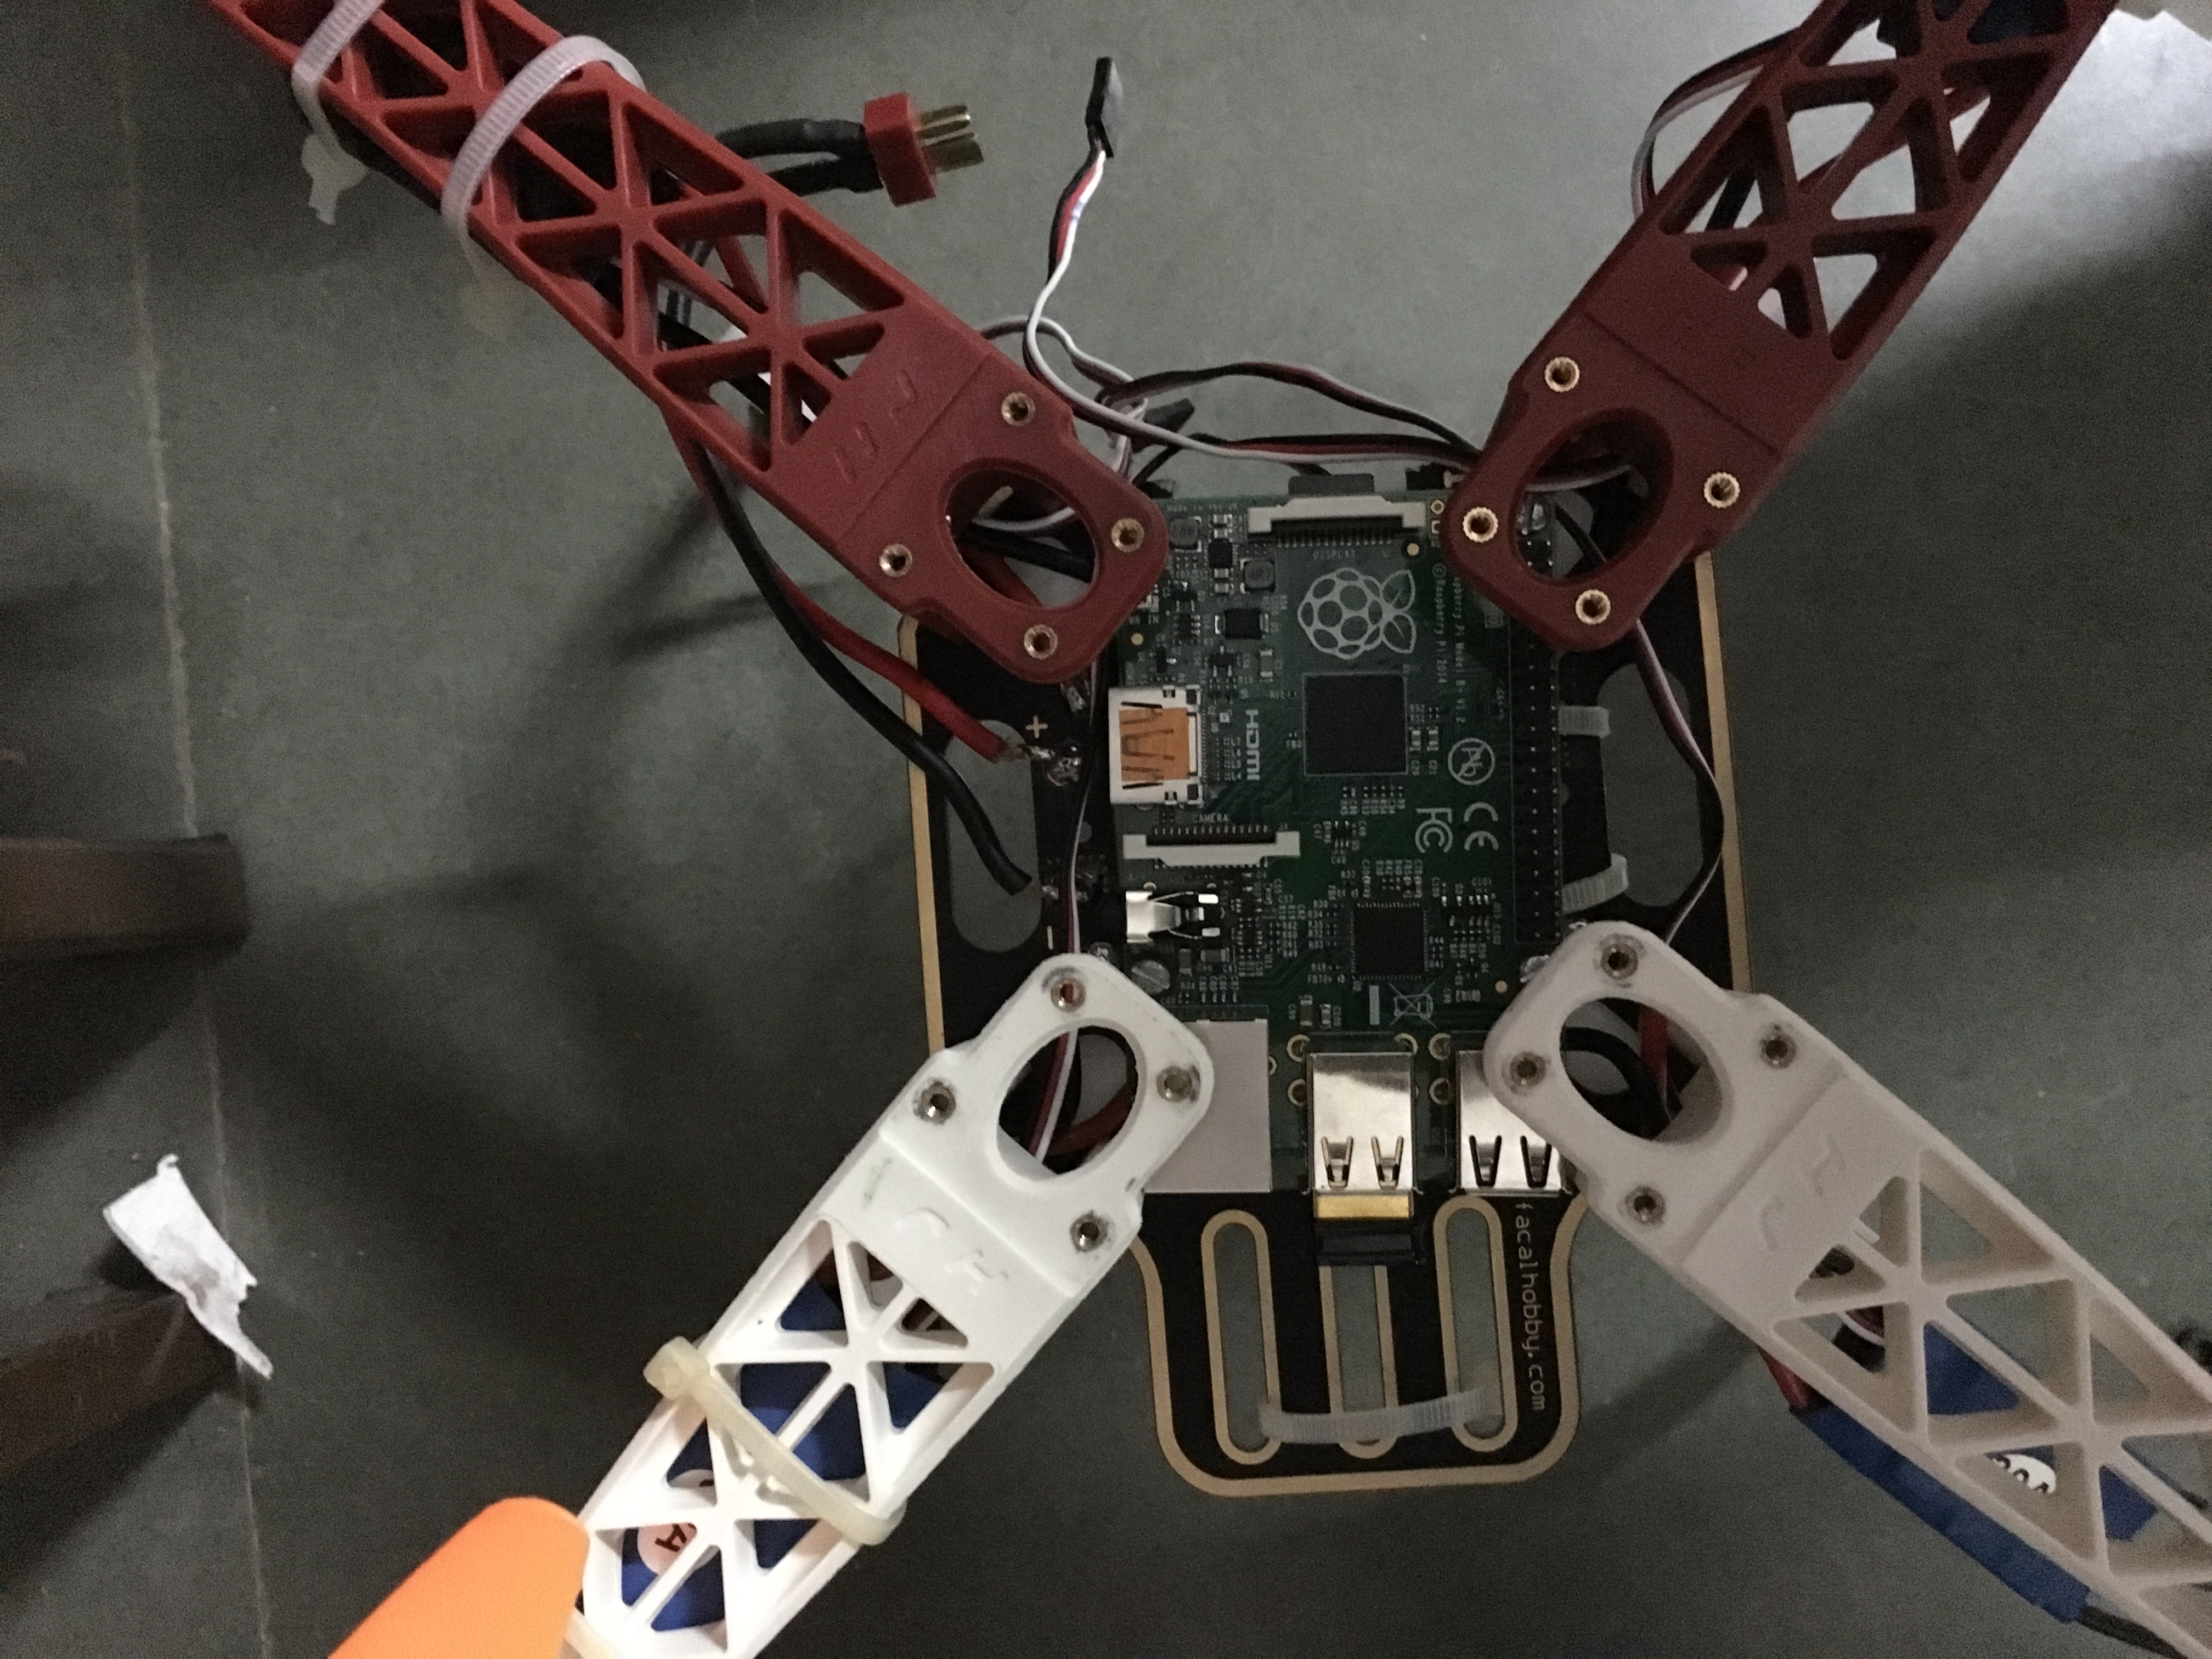
\includegraphics[scale=0.10]{Rpi}
	 	\caption{R-Pi Mounted on the Frame.}
\end{figure}
	 	\subsection{Powering the Rpi from APM}
	 	The below figure shows how to power the Rpi from the APM board by connecting a pin on positive rail on the ESC side to the UART +ve pin, and ensure that the ground pin of UART on Rpi is connected to ground of UART on Telemetry port of APM and not at Ground pin of ESC.
	 	\begin{figure}[H]
	 	\centering
		\includegraphics[scale=0.10]{apm}
	 	\caption{R-Pi Mounted on the Frame.}
\end{figure}
\end{document}



